\subsection{Approximating the distance function}
\label{sec:dist smoothing}
To create a smooth approximation to $\robf$, we use smooth approximations to each of its non-differentiable components: the set-distance, min, and max functions.

Recall that for a set $U \subset \Re^n$, $\dist(x,U) = \inf_{a \in \cl{U}} |x-a|_2$, where $|\cdot|_2$ is the Euclidian norm.
This function is globally Lipschitz with Lipschitz constant 1 and therefore differentiable almost everywhere (Rademacher's theorem), and has a second derivative almost everywhere if $U$ is convex (Alexandrov's theorem) \cite{MakelaN92book}.

It is well-known that if an a.e.-differentiable function is convolved with a smooth kernel, the output function no longer has those singularities.
We leverage this to provide a smooth approximation of the distance function by expanding it over a basis of orthonormal Meyer wavelets.
Specifically, the 1-D Meyer wavelet function is given in the frequency domain by ($i = \sqrt{-1})$:
\[\widehat{\psi}(\omega) = \frac{1}{\sqrt{2\pi}} \left \lbrace 
\begin{matrix} \sin (\frac{\pi}{2}\nu(\frac{3|\omega|}{2\pi}-1))e^{i\omega/2} & 2\pi/3 \leq |\omega| \leq 4\pi/3 \\
\cos (\frac{\pi}{2}\nu(\frac{3|\omega|}{4\pi}-1))e^{i\omega/2}, & 4\pi/3 \leq |\omega| \leq 8\pi/3\\
0, &\text{otherwise}\end{matrix} \right. \]
where $\nu(x) = 0$ if $x\leq 0$, $1$ if $x \geq 1$, and equals $x$ if $0\leq x \leq 1$.
The time-domain expression for this wavelet is given in~\cite{Valenzuela15}.
To obtain an $n$-D wavelet, we use the tensor product construction~\cite{MallatBook}.
Let $E$ be the set of vertices of the unit hypercube $[0,1]^n$.
For every $e = (e_1,e_2,\ldots,e_n) \in E$ and $x = (x_1,\ldots,x_n) \in \Re^n$, define $\Psi^e:\Re^n \rightarrow \Re$
\begin{equation*}
\label{eq:tensor meyer}
\Psi^e(x)= \psi^{e_1}(x_1)\ldots \psi^{e_n}(x_n)
\end{equation*}
Given $k \in \Ze$ and $j \in \Ze^n$, a \textit{dyadic cube} in $\Re^n$ is a set of the form $I = 2^{-k}(j + [0,1]^n)$.
Let $D$ be the set of all dyadic cubes in $\Re^n$ obtained by varying $k$ over $\Ze$ and $j$ over $\Ze^n$.
Then $\{\Psi^e_{I}, e \in E, I\in D\}$ is an orthonormal basis for $L_2(\Re^n)$ (because the Meyer wavelet itself is orthonormal).
Then every function in $L_2(\Re^n)$ has an expansion 
\[f(x) = \sum_{I \in D} \sum_{e \in E} c_I^e \Psi^e_I(x), \, c_I^e \defeq\, \langle f,\Psi^e_I \rangle\]
with $\langle h,g \rangle \defeq \int_{\Re^n}f(x)g(x)dx$.
The desired approximation is obtained by truncating this expansion after a finite number of terms, i.e., by using  a \textit{finite} set $D' \subsetneq D$
\begin{equation}
\dist(x,U) \approx \sdist(x,U) \defeq \sum_{I \in D'} \sum_{e \in E} c_I^e \Psi^e_I(x)
\end{equation}
The coefficients $c_I^e \defeq\, \langle \dist(\cdot, U), \Psi^e_I \rangle$ are calculated offline and stored in a lookup table for online usage.
Using more coefficients yields a better approximation.

%The Meyer scaling function is given in the frequency domain by 
%\[\widehat{\varphi}(\omega) = \frac{1}{\sqrt{2\pi}} \left \lbrace 
%\begin{matrix} 1 & |\omega| \leq 2\pi/3 \\
%                     \cos[\frac{\pi}{2} \nu(3|\omega|/2\pi -1)], & 2\pi/3 \leq |\omega| \leq 4\pi/3\\
%                     0, &\text{otherwise}\end{matrix} \right. \]
%where $\nu(x) = 0$ if $x\leq 0$, $1$ if $x \geq 1$, and equals $x$ if $0\leq x \leq 1$.

%They are used extensively in signal processing, because their approximation properties can be tailored to the class of functions being approximated - e.g., hyperbolic wavelets are suitable for approximating functions of mixed smoothness, such as the distance function we are interested in~\cite{Heping04_HyperbolicWav}.
%In our case, since we know the singularity lines of $\dist$, we can use a directional wavelet basis, and orient it locally such that it has slow variation along the singularity line, and fast variation accross it.


%We give an example of such a construction, which lays the groundwork for explaining the more general wavelet-based smoothing we use in the experiments.
%$C^\infty(\Re^n)$ is the class of functions that are infinitely differentiable in $\Re^n$.
%\begin{theorem}
%	\label{thm:ge smoothing}
%	Consider the globally Lipschitz function $f:\Re^n \rightarrow \Re$ with Lipschitz constant $L_f$.
%	Let $g: \Re^n \rightarrow \Re_+$ be a non-negative $C^\infty(\Re^n)$ function that integrates to 1 and is supported on the unit ball:
%	$\int_{\Re^n}g(x)dx = 1$, $g(x) = 0$ if $x \notin B(0,1)$.
%	Define $g_\varepsilon = \varepsilon^{-n}g(x/\varepsilon)$ and
%	\[f_\varepsilon(x) = f *g_\varepsilon(x) = \int_{\Re^n}f(y)g_\varepsilon(x-y)dy\]
%	Then $\fe$ is infinitely differentiable, its Lipschitz constant $L_{\fe} \leq L_f$ and $\|f-\fe\|_\infty \leq L_f \varepsilon$.
%\end{theorem}
%\begin{proof}
%	Clearly, $\fe$ is $C^\infty$: $g_\varepsilon \in C^\infty$ and the integrand in the above convolution is differentiable w.r.t. $x$, so it holds that $\fe'(x) = \int{f(y)\partial g_\varepsilon(x-y)/\partial x dy}$.
%	
%	Convolution is commutative so $f_\varepsilon(x) = \int_{\Re^n}f(x-y)g_\varepsilon(y)dy$.
%	Let $x' \in \Re^n$, then 
%	\begin{eqnarray*}
%	|\fe(x)-\fe(x')| &=& |\int_{\Re^n} f(x-y)g_\varepsilon(y) - f(x'-y)g_\varepsilon(y) dy|
%	\\
%	&\leq & \int_{\Re^n} g_\varepsilon(y)|f(x-y) - f(x'-y)| dy
%	\\
%	& = & L_f|x-x'| \int_{\Re^n} \varepsilon^{-n} g(y/\varepsilon) dy
%	\\
%	&= &L_f|x-x'| \int_{\Re^n} \varepsilon^{-n} g(y') \varepsilon^ndy'
%	\\
%	&=& L_f|x-x'| \implies L_f \leq L_{\fe}
%	\end{eqnarray*}
%	
%	Finally, 
%	\begin{eqnarray*}
%	|\fe(x)-f(x)| &=& \left|\int_{\Re^n}f(x-y)g_\varepsilon(y)dy - \int_{\Re^n}f(x)g(y)dy\right|
%	\\
%	&=& \left|\int_{\Re^n}f(x-\varepsilon y)g(y)dy - \int_{\Re^n}f(x)g(y)dy\right|
%	\\
%	&\leq& \int_{B(0,1)}|f(x- \varepsilon y) - f(x)|g(y)dy	
%	\\
%	&\leq & \int_{B(0,1)}L_f | \varepsilon y| g(y)dy \leq L_f \varepsilon
%	\end{eqnarray*}
%	In particular, $\|f-\fe\|_\infty \rightarrow 0$ as $\varepsilon \rightarrow 0$.
%\end{proof}
%Fig.~\ref{fig:smooth2d} shows the distance function $\dist(\cdot,U)$ where $U$ is a square in the plane, smoothed by convolving with kernel $g_{\varepsilon}$ obtained from the shown function. 
%We used $\varepsilon = 0.001$, and the actual approximation error $\|f-\fe\|_\infty$ is less than 1e-15.
%Parameter $\varepsilon$ controls how peaked or flat $g_\varepsilon$ is: a large $\varepsilon$ gives a peaked kernel which yields better local approximation, but the max error decreases towards 0 slower.
%
%\begin{figure}[t!]
%	\centering
%	\begin{subfigure}[t]{0.25\textwidth}
%		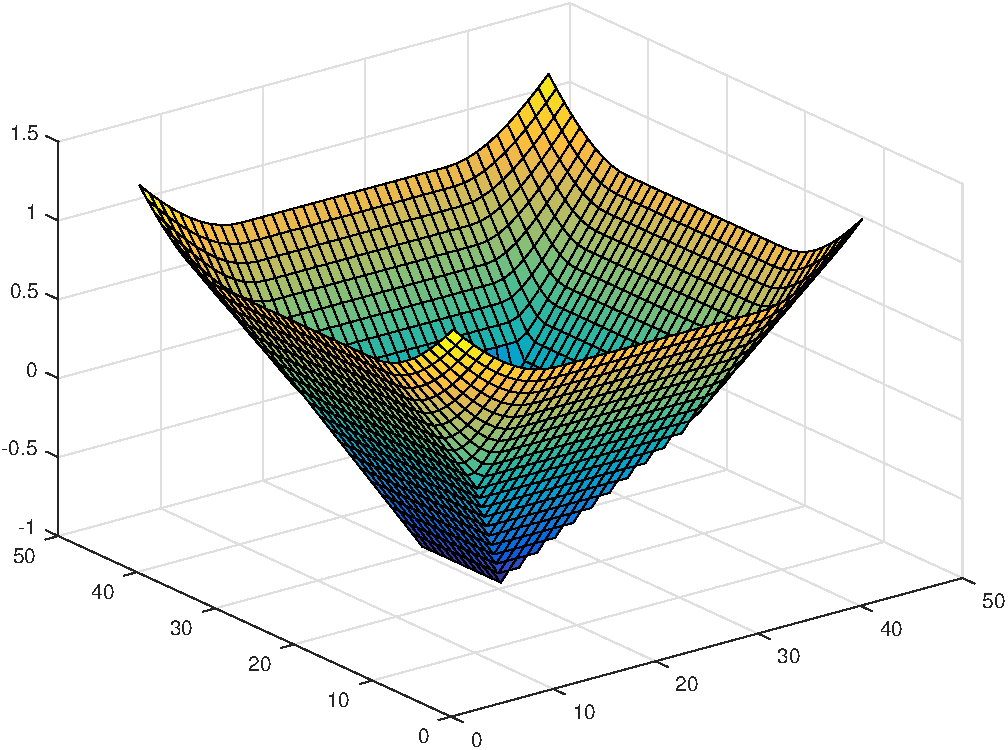
\includegraphics[height=1.2in]{figures/smoothedSignedDist}
%		\caption{Smoothed function}
%	\end{subfigure}%
%	~
%	\begin{subfigure}[t]{0.25\textwidth}
%		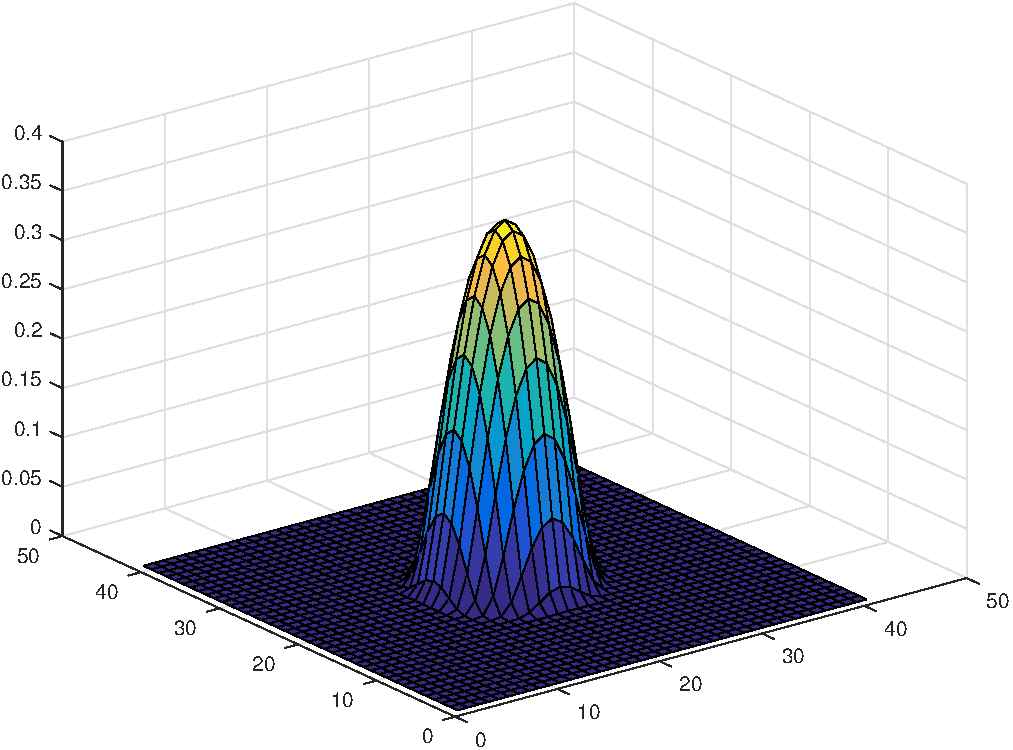
\includegraphics[height=1.2in]{figures/kernelG}
%		\caption{Function $g$}
%	\end{subfigure}
%	\caption{{\small Smoothed 2-d  (negative) signed distance function to a square in the x-y plane, and the function $g$ used to smoothen it.}}
%	\vspace{-10pt}
%	\label{fig:smooth2d}
%\end{figure}

